\subsection{Passing Pointers to Functions}
\begin{itemize}
	\item Pointers can be arguments to functions. For example, suppose you want a function that adds one to an integer argument passed by reference:
\begin{lstlisting}[style=C++]
void add_one(int *x){
	// MODIFIES: *x
	// EFFECTS: adds one to *x
	*x = *x + 1;
}
\end{lstlisting}
	\item If you were to call this function as so: \lstinline[style=C++]{add_one(bar);}, where \lstinline[style=C++]{bar} is a pointer to \lstinline[style=C++]{foo}
\begin{lstlisting}[style=C++]
int foo;
int *bar;
bar = &foo;

add_one(bar);
\end{lstlisting}
	\begin{itemize}
		\item The variable bar is bassed by \textbf{value}, but it's a pointer!
		\item Both bar and the copy of bar refer to the same address in memory.
	\end{itemize}
	\item You can also make the call without the ``middleman'' like: \lstinline[style=C++]{add_one(&foo);}
\end{itemize}

\subsection{Pointer question}
\begin{itemize}
	\item If you modify \lstinline[style=C++]{add_one} to:
\begin{lstlisting}[style=C++]
void add_one(int *x){
	x = x + 1;
}
\end{lstlisting}	
	\item It will increment the value \textbf{of the pointer} by one.
	\item Pointer arithmetic is done based on units of the \textbf{referent type} (the type of the objects in the list).
\end{itemize}

\subsection{Pointers vs. references}
\begin{itemize}
	\item Both allow you to pass objects by reference.
	\item Pointers require some extra syntax at calling time (\&), in the argument list (*), and with each use (*); references only require extra syntax in the argument list (\&).
	\item You can change the object to which a pointer points using arithmetic/assignment, but you cannot change the object to which a reference refers.
	\item You might wonder why you’d ever want to use pointers, since theyrequire extra typing, and allow you to shoot yourself in the foot.
	\item Why use pointers?
	\begin{itemize}
		\item Array variables are internally implemented using pointers
		\item They allow us to create structures (unlike arrays) whose size is not known in advance; we won't see that use until the last third of the course.
	\end{itemize}
\end{itemize}

\subsection{Pointers and Arrays}
\begin{itemize}
	\item Arrays are actually represented via pointers as so:
	\begin{center}
		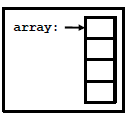
\includegraphics{sections/lec7/array.png}
	\end{center}
	\item If you were to look at the value of the variable ``array'' (not \lstinline[style=C++]{array[0]}) you'd find that it was exactly the same as the address of \lstinline[style=C++]{array[0]}.
	\item When the argument \lstinline[style=C++]{array} is passed to the function sum, a pointer to the first element of the array is really passed and the compiler does all the work of translating something like: \lstinline[style=C++]{array[3]} into the proper arithmetic/dereference to get the right value.
\begin{lstlisting}[style=C++]
x = array[3];
// Is equivalent to:
int *tmp;
tmp = array + 3;
x = *tmp;
// Or simply:
x = *(array + 3);
\end{lstlisting}
\end{itemize}

\subsection{Indexing vs. pointer arithmetic}
\begin{itemize}
	\item Using array indexing:
\begin{lstlisting}[style=C++]
for (int i = 0; i < SIZE; ++i){
	cout << array[i] << " ";
}
\end{lstlisting}
	\item Using pointer arithmetic:
\begin{lstlisting}[style=C++]
for (int *i = array; i < array+SIZE; ++i){
	cout << *i << " ";
}
\end{lstlisting}
\end{itemize}

\subsection{Array Traversal Using Pointers}
\begin{lstlisting}[style=C++]
int strlen(char *s) {
	char *p = s;
	while (*p) ++p;
	return p - s;
}
\end{lstlisting}
\begin{itemize}
	\item \lstinline[style=C++]{*p} evalues to ``false'' if \lstinline[style=C++]{p} points to a NULL, true otherwise.
	\item \lstinline[style=C++]{++p} advances by ``one character''
	\item \lstinline[style=C++]{p-s} computes the ``number of characters'' between \lstinline[style=C++]{p} and \lstinline[style=C++]{s}
\end{itemize}

\subsection{Constants}
\begin{itemize}
	\item \lstinline[style=C++]{void strcpy(char *dest, const char *src);}
	\item \lstinline[style=C++]{const} is a \textbf{type qualifier} - something that modifies a type
	\item It means ``you cannot change this value once you have initialized it.''
	\item When you have pointers, there are two things you might change:
	\begin{itemize}
		\item The value of the pointer.
		\item The value of the object to which the pointer points.
	\end{itemize}
	\item Either (or both) can be made unchangeable:
\begin{lstlisting}[style=C++]
const T *p;			// "T" (the pointed-to object) cannot be changed
T *const p;			// "p" (the pointer) cannot be changed
const T *const p;	// neither can be changed.
\end{lstlisting}
	\item Adding \lstinline[style=C++]{const} will stop changing value mistakes, and the compiler will catch them.
	\item You can use a pointer-to-T anywhere you expect a pointer-to-const-T, but NOT vice versa
	\item That's because code that expects a pointer-to-T might try to change the T, but this is illegal for a pointer-to-const-T.
	\item However, code that expects a pointer-to-const-T will work perfectly well for a pointer-to-T; it's just guaranteed not to try to change it.
\end{itemize}

\subsection{C strings vs. C++ strings}
\begin{center}
\begin{tabular}[breaklines=true]{p{5cm}|p{5cm}|p{5cm}}
	& C string & C++ string \\
	\hline
	Library headers & 
{\begin{lstlisting}[style=C++] 
#include <string>
\end{lstlisting}} & 
{\begin{lstlisting}[style=C++]
#include string
\end{lstlisting}}\\	
	string constant &
{\begin{lstlisting}[style=C++]
constchar* hello = "hello";
\end{lstlisting}}&
{\begin{lstlisting}[style=C++]
conststring hello = "hello";
\end{lstlisting}} \\
	length &
{\begin{lstlisting}[style=C++]
strlen(hello);//5
\end{lstlisting}} &
{\begin{lstlisting}[style=C++]
hello.length();//5
\end{lstlisting}} \\
	local variable &
{\begin{lstlisting}[style=C++]
constintMAXSIZE=1024; 
char s[MAXSIZE];
\end{lstlisting}} &
{\begin{lstlisting}[style=C++]
string s;
\end{lstlisting}} \\
	copy &
{\begin{lstlisting}[style=C++]
strcpy(s, hello);
\end{lstlisting}} &
{\begin{lstlisting}[style=C++]
s = hello;
\end{lstlisting}} \\
	concatenate &
{\begin{lstlisting}[style=C++]
constchar* world = " world";
char message[MAXSIZE];
strcpy(message, hello);
strcat(message, world);
\end{lstlisting}} &
{\begin{lstlisting}[style=C++]
string message = hello + " world";
\end{lstlisting}} \\
	compare &
{\begin{lstlisting}[style=C++]
if (strcmp(a,b) == 0)
	// do something
\end{lstlisting}} &
{\begin{lstlisting}[style=C++]
if (a == b)
	// do something
\end{lstlisting}} \\
	convert to C++ string &
{\begin{lstlisting}[style=C++]
string cpp_str = hello;
\end{lstlisting}} &
{\begin{lstlisting}[style=C++]
char c_str[MAXSIZE];
strcpy(c_str, message.c_str());
\end{lstlisting}} \\
\end{tabular}
\end{center}

\subsection{Type Sizes}
\begin{itemize}
	\item The amount of memory assigned to a data type is a source of innumerable ``portability bugs'' in programs.
	\item There are \textbf{some} guarantees, however:
	\begin{itemize}
		\item A ``char'' is always one byte
		\item A ``short'' is always at least as big as a char
		\item An ``int'' is always at least as big as a short
		\item A ``long'' is always at least as big as an int
	\end{itemize}
	\item \lstinline[style=C++]{sizeof(int)} tells you the number of bytes required to store an \lstinline[style=C++]{int}
	\begin{center}
		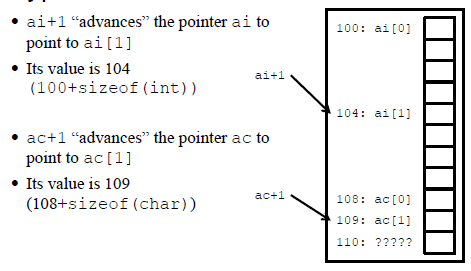
\includegraphics{sections/lec7/type.png}
	\end{center}
\end{itemize}